\documentclass{article}
\usepackage[utf8]{vietnam}
\usepackage{setspace}
\usepackage{amsmath}
\usepackage{graphicx}
\setstretch{1.2}
\doublespacing
\usepackage[linesnumbered, ruled, vlined]{algorithm2e}
\begin{document}
	\begin{center}
		\textbf{\large Chứng minh sự tương đương}
	\end{center}
	\begin{flushleft}
		\section{Kiến thức cơ sở}
			X là một tập hợp, số phần tử của X hay còn gọi là kích thước của tập hợp X được kí hiệu là |X|. Gọi $D_x$ là miền giá trị của tập hợp X. Với X là tập các biến logic, |X| = 2, $D_x$ = \{T, F\}. Một hàm logic $\theta(x)$ được định nghĩa như sau: $\theta(x)$: $B^{|x|}$ $\to$ B.\\
			Phép gán $\upsilon$ được định nghĩa như sau: $\upsilon: x \to$ B, với $D_B$ = True, $D_x$ = \{T, F\}.\\
			Gọi $\psi(\bf x, \bf x')$ là một hàm logic với với 2 biến $\bf x$, $\bf x'$. Nếu $\upsilon$ và $\upsilon'$ là các phép gán thì $\psi[\upsilon, \upsilon']$ là phép gán của $\psi$ bằng việc thay thế một cách tương ứng các $x \in \bf x$ bằng $\upsilon(x)$ và các $x' \in \bf x'$ bằng $\upsilon'(x)$. Ví dụ, giả sử $\upsilon(x) = T$ và $\upsilon'(x) = T$, nếu $\phi(x) = \overline x$ thì $\phi [\upsilon] = T$ và $\phi[\upsilon'] = F$. Nếu $\psi(x, x') = \overline x \land x'$ thì $\psi[\upsilon, \upsilon'] = T \land T = T$ và $\psi[\upsilon', \upsilon] = F \land F = F$. [1]
		\section{Dạng đặc tả được biểu diễn bởi hệ chuyển trạng thái gắn nhãn LTS}
			\subsection{Khái niệm}
				Hệ chuyển trạng thái gắn nhãn (Labeled Transition System) được định nghĩa: $S = <Q, \Sigma, \delta, q_{0}>$\\
				Trong đó:\\
				\begin{itemize}
					\item Q là tập các trạng thái của LTS, Q = $\{q_{0}, q_{1}, ..., q_{n-1}, q_{n}\}$.
					\item $\Sigma$ là tập các sự kiện của LTS, $\Sigma = \{w_{0}, w_{1}, ..., w_{n}\}$.
					\item $\delta$ là hàm chuyển trạng thái của LTS, đầu vào của  $\delta$ là một trạng thái của Q và một sự kiện của $\Sigma$, đầu ra của $\delta$ cũng là một trạng thái của Q. Với $\forall w \in \Sigma, \forall q \in Q_{1}, \forall q' \in Q_{2}$, $\delta = Q_{1} \times \Sigma \times Q_{2}$ hay $\delta(q, w) = q'$.
					\item $q_{0}$ là trạng thái khởi tạo.\\
				\end{itemize}
				Chuỗi các sự kiện được tạo thành từ các phần tử thuộc $\Sigma$ là một dãy hữu hạn các kí tự trên $\Sigma$ mà chúng được viết liền với nhau.
				Tập hợp các chuỗi được tạo thành từ $\Sigma$ được gọi là $\Sigma^*$. Ví dụ: $w_{0}, w_{0}w_{1}, w_{0}w_{1}...w_{n-1}$, ..., $w_{0}w_{1}w_{2}...w_{n}$.\\
				Hàm chuyển trạng thái mở rộng của trạng thái q được kí hiệu là $\delta^*$ là một hàm nhận đầu vào là một xâu $\alpha \in \Sigma^*$, trạng thái $q \in Q_{1}$ và đầu ra là $q_{i} \in Q_2$ với $\forall q_{i} \in Q_{2}$ hay $\delta^*(q, \alpha) = q_{i}$.
				Ngôn ngữ của hệ chuyển trạng thái gắn nhãn (LTS) S được kí hiệu là L(S) được định nghĩa như sau:
				$L(S) = \{\alpha \in \Sigma^* | \delta^*(q_{0}, \alpha) = q_i \in Q_{2}\}$\\
		\section{Dạng đặc tả sử dụng hàm logic (Bool)}
			\subsection{Khái niệm}
			Dạng đặc tả sử dụng hàm logic được biểu diễn như sau: \\
				$B = <X, E, \tau(x, e, x'), \iota(x)>$\\
				Trong đó:\\
				\begin{itemize}
					\item X là tập các biến logic dùng để biểu diễn các trạng thái của hệ thống. X = $\{x_0, x_1, ..., x_n\}$
					\item E là tập các biến logic dùng để biểu diễn các tác nhân tác động vào hệ thống. E = $\{e_0, e_1, ..., e_{n-1}\}$
					\item $\tau(x, e, x')$ là hàm logic biểu diễn việc chuyển trạng thái của hệ thống, với $\forall x, x' \in X$ và $\forall e \in E$. Ta luôn có:
					$\tau(x, e, x')$ = $X \land E \land X$.
					\item $\iota(x)$ là hàm logic dùng để biểu diễn các trạng thái khởi tạo của hệ thống.
				\end{itemize}
				Với $\tau(x, e, x')$ là hàm logic biểu diễn việc chuyển trạng thái của hệ thống, xét một chuyển trạng thái thứ i bất kì, khi $\tau[x_i, e_i, x_{i+1}]$ = True là một bộ 3 các phép gán cho các hàm mã hóa $x_i, e_i, x_{i+1}$ thì $\upsilon[x_i]$ = True, $\upsilon[e_i]$ = True và $\upsilon[x_{i+1}]$ = True. Chuỗi hữu hạn các phép gán cho hàm mã hóa các sự kiện $\sigma = \upsilon(e_0)\upsilon(e_1)...\upsilon(e_{n-1})$ được gọi là Trace của B. Khi đó, $\iota[\upsilon^0]$ = True và $\tau[\upsilon^i, \upsilon^{i+1}]$ = True với $\forall i: 0 \leq i < n$.\\
				Tập các trace của B được gọi là ngôn ngữ của B, kí hiệu là L(B), $L(B) = \{\sigma\ |\ \sigma$ là một trace của B\}\\
		\section{Phương pháp chuyển đổi}
		\subsection{Khái niệm về bảng ánh xạ}
			Bảng ánh xạ (mapping) là một bảng dùng để lưu lại các ánh xạ khi chuyển đổi từ dạng đặc tả sử dụng LTS sang dạng đặc tả sử dụng hàm logic và ngược lại.\\
			Gọi Map là kí hiệu của bảng ánh xạ. Với một LTS $S = <Q, \Sigma, \delta, q_{0}>$ và một dạng đặc tả sử dụng hàm logic $B = <X, E, \tau(x, e, x'), \iota(x)>$. Ta định nghĩa:\\
			Map = $\{Q = Q_1 \cup Q_2, \Sigma, \delta(q, e, q'), X = X_1 \cup X_2, E, \tau(x, e, x')\}$\\
			Trong đó:\\
			$Q = Q_1 \cup Q_2$ là tập các trang thái của LTS. Với $Q_1$ là tập các trạng thái đầu vào (from), $Q_2$ là tập các trạng thái đầu ra (to).\\
			\item $\Sigma$ là tập các sự kiện của LTS.\\
			\item $\delta$ là hàm chuyển trạng thái.\\
			$X = X_1 \cup X_2$ là dạng đặc tả sử dụng hàm logic của tập các trạng thái. Với $X_1$, $X_2$ lần lượt là dạng đặc tả sử dụng hàm logic của tập các trạng thái đầu vào và đầu ra.\\
			\item E là tập các biến logic dùng để biểu diễn các tác nhân tác động vào hệ thống, E = $\{e_0, e_1, ..., e_{n-1}\}$
			\item $\tau(x, e, x')$ là dạng đặc tả sử dụng hàm logic của tập các chuyển trạng thái của hệ thống.\\
			Ví dụ: Với một LTS như hình vẽ. Ta có tập các trạng thái $Q = \{a, b, c\}$. Với tập các trạng thái đầu vào $Q_{1} = \{a, b, c\}$, tập trạng thái đầu ra $Q_{2} = \{b, c, a\}$ và tập các sự kiện $E = \{send, out, ack\}$.\\
			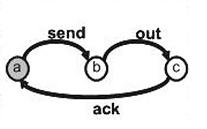
\includegraphics{hinh1.png}\\
			Ta có bảng ánh xạ:
			\begin{table}[!ht]
				\centering
				\renewcommand{\arraystretch}{1.25}
				\begin{tabular}{|c|c|c|c|c|}
					\hline
					$Q_1$ & a & b & c\\
					\hline
					$X_1$ & $x_0x_1$ & $x_0\overline x_1$& $\overline x_0x_1$\\
					\hline
				\end{tabular}
				\begin{tabular}{|c|c|c|c|c|}
					\hline
					$Q_2$ & a & b & c\\
					\hline
					$X_2$ & $x_4x_5$ & $x_4\overline x_5$& $\overline x_4x_5$\\
					\hline
				\end{tabular}
			\end{table}
			\begin{table}[!ht]
				\centering
				\renewcommand{\arraystretch}{1.25}
				\begin{tabular}{|c|c|c|c|}
					\hline
					$\Sigma$ & send & out & ack\\
					\hline
					E & $x_2x_3$ & $x_2\overline x_3$& $\overline x_2x_3$ \\
					\hline
				\end{tabular}
			\end{table}
			\begin{table}[!ht]
				\centering
				\renewcommand{\arraystretch}{1.25}
				\begin{tabular}{|c|c|c|c|}
					\hline
					$\delta(q, e, q')$ & $\delta(a, send, b)$ & $\delta(b, out, c)$ & $\delta(c, ack, a)$\\
					\hline
					$\tau(x, e, x')$ & $x_0x_1 \land x_2x_3 \land x_4\overline x_5$ & $x_0\overline x_1 \land x_2 \overline x_3 \land x_4 \overline x_5$ & $\overline x_0 x_1 \land \overline x_2 x_3 \land x_4x_5$ \\
					\hline
				\end{tabular}
				\caption{Ví dụ về bảng ánh xạ}
			\end{table}				
		\subsection{Thuật toán}
		Đầu vào (Input): Một hệ chuyển trạng thái gắn nhãn (LTS).\\
		Đầu ra (Output): Dạng đặc tả sử dụng hàm logic.\\
		Thuật toán chia làm 3 bước:
		
		\begin{itemize}
			\item Bước 1: Mã hóa tập các trạng thái.
			\item Bước 2: Mã hóa tập các sự kiện.
			\item Bước 3: Mã hóa tập các chuyển trạng thái.
		\end{itemize}
		
		\begin{algorithm}[H]
			\SetAlgoLined
			\DontPrintSemicolon
			\KwData{Tập các trạng thái của LTS.}
			\KwResult{Tập các trạng thái được biểu diễn bằng dạng đặc tả sử dụng hàm logic.}
				
			\For{mỗi trạng thái $q_{i}$ trong tập các trạng thái Q}{
				x = True\;
				k = Thứ tự của $q_i$ trong Q\;
				Chuyển k sang số nhị phân với độ dài $|Q| + 1$ bit\;
				\For{mỗi bit $x_i$ trong chuỗi nhị phân biểu diễn k} {
					\uIf{$x_i$ = 1} {
						Biểu diễn $x_i$ dưới dạng $x_i$\;
					}
					\Else {
						Biểu diễn $x_i$ dưới dạng $\overline x_i$\;
					}
					$x = \lor_{i=1}^n \{x_i \land x\}$
				}
				Lưu x vào bảng ánh xạ ứng với vị trí của $q_i$.
			}
			\caption{Mã hóa tập các trạng thái}
		\end{algorithm}
		\begin{algorithm}[H]
			\SetAlgoLined
			\DontPrintSemicolon
			\KwData{Tập các sự kiện của LTS.}
			\KwResult{Tập các sự kiện biểu diễn bằng dạng đặc tả sử dụng hàm logic.}
				
			\For{mỗi sự kiện $w_i$ trong tập các sự kiện $\Sigma$}{
				e = True\;
				k = Thứ tự của $w_i$ trong $\Sigma$\;
				Chuyển k sang số nhị phân với độ dài $|\Sigma| + 1$ bit\;
				\For{mỗi bit $x_i$ trong chuỗi nhị phân biểu diễn k} {
					\uIf{$x_i$ = 1} {
						Biểu diễn $x_i$ dưới dạng $x_i$\;
					}
					\Else {
						Biểu diễn $x_i$ dưới dạng $\overline x_i$\;
					}
					$e = \lor_{i=1}^n \{x_i \land e\}$
				}
				Lưu e vào bảng ánh xạ ứng với vị trí của $w_i$
			}
			\caption{Mã hóa tập các sự kiện}
		\end{algorithm}
		\begin{algorithm}[H]
			\SetAlgoLined
			\DontPrintSemicolon
			\KwData{Tập các chuyển trạng thái của LTS.}
			\KwResult{Tập các chuyển trạng thái được biểu diễn bằng dạng đặc tả sử dụng hàm logic.}
				
			\For{mỗi chuyển trạng thái được biểu diễn $\delta(\textit{from}, \textit{event}) = \textit{to}$ của LTS}{
				Lấy dạng biểu diễn của \textit{from} từ bảng ánh xạ\;
				Lấy dạng biểu diễn của \textit{event} từ bảng ánh xạ\;
				Lấy dạng biểu diễn của \textit{to} từ bảng ánh xạ\;
				Biểu diễn chuyển trạng thái dươi dạng: $x_i\land e_i \land x_{i+1}$
			}
			\Return $\tau = \lor_{i=1}^n \{x_i \land e_i \land x_{i+1}\}$
				
			\caption{Mã hóa tập các chuyển trạng thái}
		\end{algorithm}

		Với thuật toán mã hóa 3, đầu ra của thuật toán này là $\tau = \lor_{i=1}^n \{x_i \land e_i \land x_{i+1}\}$. Xét $\tau_i = \{x_i \land e_i \land x_{i+1}\}$, $\tau_j = \{x_j \land e_j \land x_{j+1}\}$ với j = i + 1, ta có $\psi [\tau_i]$ = True thì $\upsilon[x_i]$ = True, $\upsilon[x_{i+1}]$ = True, $\upsilon[e_i]$ = True, $\psi [\tau_j]$ = True thì $\upsilon[x_j]$ = True, $\upsilon[x_{j+1}]$ = True, $\upsilon[e_j]$ = True, khi đó $\tau [e_i, e_j]$ = True.
		\subsection{Mã hóa các trạng thái và các sự kiện (Event)}
		Với Q là tập các trạng thái của LTS, $Q = Q_1 \cup Q_2$, với $Q_1$ là tập các trạng thái đầu vào (from) và $Q_2$ tập các trạng thái đầu ra (to).\\
		Xét tập $Q_{1} = S_{1}, S_{2}, ..., S_{n}$ (n trạng thái), |$Q_{1}$| = n. Số biến logic cần dùng để mã hóa tập các trạng thái $Q_{1}$ là $[log_{2}n] + 1$ = m.\\
		Gọi $x_{1}, x_{2}, ..., x_{m}$ là chuỗi biến logic dùng để mã hóa các trạng thái trong $Q_{1}$. Mỗi trạng thái $S_{i}$ trong $Q_{1}$ sẽ được biểu diễn dưới dạng $x_{1}\land x_{2}\land...\land x_{m}$.\\
		Xét trạng thái bất kì $S_{k}$ trong tập $Q_{1}$, theo bước (2) ta xác định được thứ tự của $S_{k}$ trong tập $Q_{1}$ là k, theo bước (3) sẽ biểu diễn k dưới dạng số nhị phân $[log_{2}n] + 1$ bit. Theo bước (4)-(10) chúng ta biểu diễn được trạng thái $Q_{i}$ sang dạng đặc tả sử dụng bằng hàm logic. Theo bước (11) dạng biểu diễn của trạng thái $S_k$ sẽ được lưu vào trong bảng ánh xạ. Mục đích của việc lưu vào bảng ánh xạ là để dùng cho việc chuyển ngược lại từ dạng đặc tả sử dụng hàm logic sang dạng đặc tả sử dụng LTS. Mặt khác, thứ tự của mỗi trạng thái trong $Q_1$ là duy nhất nên dạng biểu diễn của mỗi trang thái trong $Q_1$ là duy nhất.\\
		Một cách tương tự cho các trạng thái khác, chúng ta sẽ mã hóa tất cả các trạng thái trong tập trạng thái đầu vào $Q_{1}$. Thêm vào đó, sau khi mã hóa, các thông tin về trạng thái và dạng biểu diễn sử dụng hàm logic của các trạng thái này sẽ được lưu vào bảng ánh xạ, nhằm mục đích sử dụng cho việc chuyển đổi ngược lại từ dạng đặc tả sử dụng hàm logic sang dạng đặc tả sử dụng LTS.\\
		Áp dụng cách mã hóa trên cho tập trạng thái đầu ra $Q_{2}$ và tập các sự kiện $\Sigma$.
		\subsection{Mã hóa các chuyển trạng thái}
		Một chuyển trạng thái (Transition) được biểu diễn là một bộ 3 $\delta = Q_{1} \times \Sigma \times Q_{2}$ hay $\delta = q_{i} \land e_i \land q_{i+1}$ với $\forall q_{i} \in Q_{1}$, $\forall e_{i} \in \Sigma$\\ và $\forall q_{i+1} \in Q_{2}$
		Theo bước (2) trạng thái đầu vào from = $q_{i}$ sẽ được chuyển sang dạng đặc tả sử dụng hàm logic. Theo bước (3) sự kiện $e_i$ sẽ được chuyển sang dạng đặc tả sử dụng hàm logic. Theo bước (4) trạng thái đầu ra to = $q_{i+1}$ sẽ được chuyển sang dạng đặc tả sử dụng hàm logic. Sau bước (5), mỗi chuyển đổi trạng thái sẽ được biểu diễn dưới dạng $x_{i} \land e_i \land x_{i+1}$.\\
		\section{Chứng minh}
		Để chứng minh ngôn ngữ của dạng đặc tả được biểu diễn bằng LTS tương đương với ngôn ngữ của dạng đặc tả sử dụng hàm logic, chúng ta cần chứng minh 2 mệnh đề:
		\begin{itemize}
			\item Mệnh đề 1: Ngôn ngữ của dạng đặc tả hệ thống biểu diễn bằng LTS sau khi chuyển đổi sang dạng đặc tả biểu diễn bằng hàm logic được đoán nhận bởi ngôn ngữ của dạng đặc tả được biểu diễn bởi hàm logic. (1)\\
			\item Mệnh đề 2: Ngôn ngữ của dạng đặc tả được chuyển đổi từ hàm logic sau khi chuyển đổi sang dạng đặc tả biểu diễn bằng LTS được đoán nhận bởi ngôn ngữ của LTS.
		\end{itemize}
		\textbf{Chứng minh mệnh đề 1}:\\
		Gọi $\alpha = w_0w_1...w_{n-1}$ là một dẫn xuất bất kì trong ngôn ngữ L, áp dụng thuật toán mã hóa như đã trình bày ở 4.1, ta được một dẫn xuất $\alpha' = e_0e_1...e_{n-2}e_{n-1}$ và một bảng mapping A, ta sẽ chứng minh $\alpha'$ cũng được đoán nhận với ngôn ngữ của dạng đặc tả được biểu diễn bởi hàm logic.\\
		Thật vậy, vì $\alpha'$ là đầu ra của $\alpha$ trong thuật toán mã hóa, mà $w_{0}$ là sự kiện đầu tiên của LTS nên $\iota[e_0]$ = True. Mặt khác, $\delta(q_i, w_i) = q_{i+1}$, $\delta(q_{i+1}, w_{i+1}) = q_{i+2}$ với $\forall i: 0 \leq i < n$ nên $\tau[x_i, e_i, x_{i+1}]$ = True và $\tau[x_{i+1}, e_{i+1}, x_{i+2}]$ = True, $\tau[e_i, e_{i+1}]$ = True. Do đó, $\alpha'$ là một trace của B.\\
		\textbf{Chứng minh mệnh đề 2}:\\
		Gọi $\xi = e_0e_1...e_{n-1}$ là một trace của B. Gọi A là bảng ánh xạ lưu các ánh xạ khi chuyển đổi từ dạng đặc tả sử dụng LTS sang dạng đặc tả sử dụng hàm logic. Áp dụng thuật toán mã hóa đã trình bày ở 4.1, ta được một chuỗi $\xi' = w_0w_1...w_{n-2}w_{n-1}$. Ta sẽ chứng minh $\xi'$ được đoán nhận bởi LTS. Thật vậy, với $e_0$ là dạng biểu diễn cho của sự kiện thứ 0 của dạng đặc tả sử dụng hàm logic, khi đó $\iota[e_0]$ = True, dựa vào bảng ánh xạ $e_0$ tương ứng với  $w_{0}$ của dạng biểu diễn diễn sử dụng LTS do đó $w_{0}$ là sự kiện thứ 0 hay sự kiện đầu tiên của LTS. Vì $\xi$ là một trace của B nên $\tau[e_i,e_{i+1}] = T$ với $\forall i: 0 \leq i < n$, vì thế $\tau[x_i, e_i, x_{i+1}]$ = True, $\tau[x_{i+1}, e_{i+1}, x_{i+2}]$ = True. Dựa vào bảng ánh xạ, $x_i$ ứng với $q_i$, $x_{i+1}$ ứng với $q_{i+1}$, $x_{i+2}$ ứng với $q_{i+2}$, $e_i$ ứng với $w_i$, $e_{i+1}$ ứng với $w_{i+1}$ trong dạng đặc tả sử dụng LTS, do đó $\delta(q_{i}, w_{i}) = q_{i+1}$, $\delta(q_{i+1}, w_{i+1}) = q_{i+2}$ với $\forall i: 0 \leq i < n$, $\delta$ là hàm chuyển trạng thái của LTS. Ta thấy, $\xi'$ hoàn toàn được đoán nhận bởi ngôn ngữ của LTS.
	\end{flushleft}
\begin{thebibliography}{9}
	\bibitem{latexcompanion} 
	Yu-Fang Chen, Edmund M. Clarke, Azadeh Farzan, Ming-Hsien Tsai,
	Yih-Kuen Tsay, and Bow-Yaw Wang \textit{Automated Assume-Guarantee Reasoning
		through Implicit Learning}. 
	Addison-Wesley, Reading, Massachusetts, 1993.
\end{thebibliography}
\end{document}